\documentclass[a4paper,11pt]{book}

\usepackage{mystyle}
\usepackage{cite}
\usepackage{chapterbib}

\begin{document}
\selectlanguage{spanish}
\pagenumbering{gobble}
\begin{titlepage}
 
 
\newlength{\centeroffset}
\setlength{\centeroffset}{-0.5\oddsidemargin}
\addtolength{\centeroffset}{0.5\evensidemargin}
\thispagestyle{empty}

\noindent\hspace*{\centeroffset}\begin{minipage}{\textwidth}

\centering

\includegraphics[width=0.9\textwidth]{img/logo_ugr.jpg}\\[1.4cm]

\textsc{ \Large TRABAJO FIN DE GRADO\\[0.2cm]}
\textsc{ Doble Grado en Ingeniería Informática y Matemáticas}\\[1cm]
% Upper part of the page
% 
% Title
{\large\bfseries Sistema de recuperación de imágenes basado en
términos linguisticos de alto nivel semántico
\\
}
\noindent\rule[-1ex]{\textwidth}{3pt}\\[3.5ex]
\end{minipage}

\vspace{2.5cm}
\noindent\hspace*{\centeroffset}\begin{minipage}{\textwidth}
\centering

\textbf{Autor}\\ {Luis Suárez Lloréns}\\[2.5ex]
\textbf{Director}\\
{Jesús Chamorro Martínez}\\[2cm]

\includegraphics[width=0.3\textwidth]{img/logo_etsiit.png} \hfill 
\includegraphics[width=0.3\textwidth]{img/logo_ciencias.jpg}\\[0.1cm]
\textsc{---}\\
Granada, Septiembre de 2016
\end{minipage}
%\addtolength{\textwidth}{\centeroffset}
%\vspace{\stretch{2}}
\end{titlepage}

\frontmatter
\pagenumbering{gobble}

\cleardoublepage
\thispagestyle{empty}

\begin{center}
{\large\bfseries Sistema de recuperación de imágenes basado en
términos lingüísticos de alto nivel semántico}\\
\end{center}
\begin{center}
Luis Suárez Lloréns\\
\end{center}

%\vspace{0.7cm}
\noindent{\textbf{Palabras clave}: imagen, recuperación de información, forma, lógica difusa, aprendizaje automático, deep learning, red neuronal, red neuronal convolucional.}\\

\vspace{0.7cm}
\noindent{\textbf{Resumen}}\\

En la actualidad, la cantidad de información generada por el ser humano está creciendo a un ritmo muy rápido. Por ejemplo, con la fotografía digital, que elimina las limitaciones del carrete, la cantidad de imágenes en las manos de los usuarios ya empezó a crecer a gran velocidad. Este fenómeno ha crecido aún más con el crecimiento de las redes sociales, donde los usuarios depositan sus comentarios, fotos y videos.

Este crecimiento genera un nuevo problema. El usuario tiene que ser capaz de encontrar su información entre tantos ficheros. La solución es un sistema de recuperación de información que sea capaz de encontrar el fichero del usuario tras una consulta del mismo. Los buscadores de web son un claro ejemplo de este tipo de sistemas.

Este proyecto intenta crear un sistema de recuperación de imágenes, pero con una pequeña modificación. Normalmente, los sistemas de recuperación de imágenes necesitan información aportada por el usuario para realizar la búsqueda. Un ejemplo es la plataforma Instagram, donde los propios usuarios clasifican sus fotos, y luego se pueden buscar imágenes gracias a esa información. El objetivo del proyecto será que la aplicación que sea capaz de clasificar automáticamente las imágenes, sin necesidad de interacción del usuario, para después utilizar esa información generada para ser capaz de recuperar las imágenes.

Normalmente, las aplicaciones existentes de recuperación de imágenes, que usan solo información de las imágenes para buscar, tienen definido un conjunto de descriptores de la imagen. Estos descriptores se comparan a los descriptores de la imagen de consulta, para recuperar imágenes que se parezcan a la de consulta.

El objetivo es entonces transformar imágenes en palabras, y va a tratar dos enfoques del problema. Por un lado, tratar de describir las formas de un objeto y por otro, utilizar técnicas de aprendizaje automático para clasificar automáticamente imágenes.


Para el primer objetivo, usaremos la lógica difusa. En el mundo real esta lleno de imprecisiones y de diferentes puntos de vista. por ejemplo, es común considerar la esquina de una mesa como un vértice, aunque seguramente esta estará redondeada. La lógica difusa es uno de los modelos matemáticos que intenta adaptar la lógica formal al mundo real, tratando de adaptarse y modelar las imprecisiones que se encuentran en el mundo real. Por tanto, usaremos la lógica difusa para definir conceptos básicos de los contornos: ``linealidad'', ``curvacidad'' y ``verticidad''. Estos elementos se podrán usar en el futuro para definir y poder reconocer formas más complejas, como por ejemplo polígonos.  

Para el segundo objetivo, utilizaremos las técnicas de aprendizaje automático que mejores resultados han dado en las competiciones de clasificación de imágenes. Utilizaremos un modelo encajado dentro del conocido deep learning. Tradicionalmente, en los problemas de aprendizaje automático, se generaba un conjunto de características, que luego se daban como entrada a un clasificador. Los modelos de deep learinig se caracterizan por utilizar como entrada al clasificador el dato sin procesar. Es por tanto, el propio clasificador el que aprende por su cuenta las características. El tipo que clasificador que utilizaremos será una red neuronal convolucional, un tipo de red neuronal artificial. Estos modelos imitan el comportamiento de un cerebro, donde una gran cantidad de neuronas artificiales se comunican entre ellas para tratar de obtener el resultado  deseado.

La aplicación utilizará las técnicas desarrolladas en los dos apartados para recuperar imágenes dentro del ordenador del usuario, de una manera sencilla, mostrándole al usuario los resultados ordenados según el nivel de satisfacción de la consulta.
 
\cleardoublepage


\thispagestyle{empty}

\selectlanguage{USenglish}
\begin{center}
{\large\bfseries Project Title: Project Subtitle}\\
\end{center}
\begin{center}
Luis Suárez Lloréns\\
\end{center}

%\vspace{0.7cm}
\noindent{\textbf{Keywords}: Image, Information retrieval, shape, fuzzy logic, machine learning, deep learning, neural network, convolutional neural network}\\

\vspace{0.7cm}
\noindent{\textbf{Abstract}}\\

Nowadays, the amount of information and files generated by the human kind is growing way faster than we can handle. A good example of this phenomenon is the digital photography. It changed the way people used their cameras, from a few pics in every travel to hundreds of photos per day given the memory increase and ease of use this technology. Now, it is really common to store thousand of pics in our computers.  There are more examples of this new tendency.  New social media networks, like Facebook, Twitter and Instagram are clear examples of this growth. Millions of users upload their opinions, photographies and videos to this social networks. 

A problem arise from this grow of information. The user is unable to find a file or picture, even in the user’s device. The solution is an Information Retrieval system  that finds the information after a query from the user. Web search engines are the most noticeable example of this kind of applications.

This project tries to create an Information Retrieval System for pictures and photos from the user’s device, with a little twist. Usually, Information Retrieval Systems need some information to be able to search. Web search engines use text, which is a really easy type of information to use for these purposes, because is a structured type of data. For pictures, some social media network like Instagram let their users tag the images, and after that uses those tags to search the database after a query . The objective of this project is to create an application that is able to automatically generate tags for the images of the user. Then, it will use that information to show images that fulfil the user’s query. Therefore, the application needs an Artificial Intelligence to be able to do the task. 

Usually, the Information Retrieval Systems for images that only uses the information from the images to search, have defined some set of descriptors like mean color, dominant colors, texture or edges of the image. Then, all those descriptors are compared, in order to show the closest images to the query image. So this kind of Information Retrieval System transform images into a vector of values for those descriptors.

This project objective is to transform images into words. It will focus on two aspects. The first one is to define qualities of the shape of the object in order to be able to describe the shape of the object. The second one is the use of machine learning techniques, like neural networks, to classify an image into a set of categories.

The shape of an object is a really good source of information to be able to recognize the object. With only a black silhouette, we can easily distinguish two different elements. For example, the shape of a heart or the shape of a fish is really easy to recognize. Therefore, the shape must be a good descriptor of our images. But images, and the perception of the images by the people is really imprecise. For example, a person can classify a table’s corner as a vertex, another person can classify it as a no-vertex, because is too rounded to be a vertex.

So, in order to be able to modelize this reality, is necessary to introduce a new kind of logic that accept the imprecision inherent of this problem. There are lots of mathematical models trying to solve this problem. In this project, we are going to use one of them, the fuzzy set theory and fuzzy logic. The fuzzy set theory is an extension to the usual set theory. There is a major difference between the two theories. In the usual set theory, an element is either on the set or outside the set. In the fuzzy set theory, an element have a degree of membership to the set. As an example, imagine a person which height is 1.80 meters. In the usual set theory, there are only two options. Either is a tall person or he is not. It leaves no place for “is no tall enough but is not short” kind of description. Inside the fuzzy set theory, is possible to make this kind of descriptions. For example, that person will have an 0.7 membership value in the set “tall” and a 0.3 in the set “short”. This ability creates a whole new world of possibilities.

This project will describe the shape of the objects through the use of fuzzy logic. It will define the concepts “linearity”, “curvacity” and “verticity”. Those concept will be use in the future to be able to describe shapes, starting with the most simples ones, like squares and any other polygons.

The other side of the project is the use of a classifier to automatically tag the images of the user. The objective is to use machine learning techniques, among a really big set of images, to be able to learn the paterns necesary to recognize the objects in them. The state of art classifier for this task is based directly in a brain. An artificial neural network is a simplified version of a brain. In then, hundreds or thousends of artificial neurons interconect with the other, in order to process the input information into a result.

Usually, this kinds of artificial intelligence applications needed the creation of a very well designed descriptors set. But in this case, the data will be feed raw to the artificial neural network, without the creation of any descriptor. Then the multiple layers of the neural network will learn really complex descriptors automatically.  Feeding the data raw to the artificial intelligence, leaving to the system the task of the creation of the descriptors is called deep learning.

An specific type of neural network, convolutional neural network, will be used for the application. This type of neural network, introduced by Yann Lecun, has made greats advances in the field of image classification and many other field, where the data is not structurated. The idea is to search features in a window, and pass that window through all the image. For example, to find an eye in a picture, we will use a window of the proper size to find that feature, instead of searching in the image as a whole. Using that idea, Lecun was able to reduce the input to every neuron, from all the pixels in the image to only the pixels inside the window. Even more, all the neurons in the same layer will share the feature they search, so they also share the weights they use to compute. This is logical because the system does not know where the object will be in the image, and if a feature is meaningful, the system will want to find it anywhere. These little adjustments, to fit the neural networks for their use with images was a big revolution, shattering the competitors in multiple competitions of machine learning.
\selectlanguage{spanish}
\chapter*{}
\thispagestyle{empty}

\noindent\rule[-1ex]{\textwidth}{2pt}\\[4.5ex]

Yo, \textbf{L}, alumno de la titulación TITULACIÓN de la \textbf{Escuela Técnica Superior
de Ingenierías Informática y de Telecomunicación de la Universidad de Granada}, con DNI XXXXXXXXX, autorizo la
ubicación de la siguiente copia de mi Trabajo Fin de Grado en la biblioteca del centro para que pueda ser
consultada por las personas que lo deseen.

\vspace{6cm}

\noindent Fdo: Luis Suárez Lloréns

\vspace{2cm}

\begin{flushright}
Granada a X de septiembre de 2016.
\end{flushright}


\chapter*{}
\thispagestyle{empty}

\noindent\rule[-1ex]{\textwidth}{2pt}\\[4.5ex]

D. \textbf{Jesús Chamorro Martínez}, Profesor del Área de XXXX del Departamento YYYY de la Universidad de Granada.

\vspace{0.5cm}

\textbf{Informa:}

\vspace{0.5cm}

Que el presente trabajo, titulado \textit{\textbf{Sistema de recuperación de imágenes basado en
términos lingüísticos de alto nivel semántico
\\}},
ha sido realizado bajo su supervisión por \textbf{Luis Suárez Lloréns}, y autoriza la defensa de dicho trabajo ante el tribunal
que corresponda.

\vspace{0.5cm}

Y para que conste, expide y firma el presente informe en Granada a X de septiembre de 2016.

\vspace{1cm}

\textbf{El director:}

\vspace{5cm}

\noindent \textbf{Jesús Chamorro Martínez}

\chapter*{Agradecimientos}
\thispagestyle{empty}

       \vspace{1cm}


Poner aquí agradecimientos...



\tableofcontents
\listoftodos

\mainmatter
%\input{tex/abstract}
\chapter{Introducción}
\label{ch0}
\section{Introducción}
La gestión de la información generada por los seres humanos es una de las tareas fundamentales de la informática. Además de las tareas básicas esperadas de este proceso, como el almacenamiento y la edición de dicha información, se plantea también la necesidad de clasificar esta información, para facilitar el acceso rápido y eficiente a la misma.\\

Por supuesto, la clasificación puede ser realizada manualmente por los usuarios, pero este proceso se puede volver intratable cuando la cantidad de información crece de manera muy rápida. Por tanto, es necesario automatizar el proceso, y dejar que el ordenador ordene por categorías la información.\\

Esta tarea, que es compleja por sí misma, se dificulta más cuando la información no está estructurada de manera clara. El caso de estudio de este trabajo se centra en el mundo de las imágenes. Es fácil ver que, salvo algunos casos donde las imágenes se toman en un ambiente altamente controlado ---imágenes de control de calidad en una fábrica, por ejemplo---, las imágenes no tienen una estructura, ni áreas a destacar de antemano. Es más, si en la imagen aparece un animal para una persona es muy fácil reconocerlo, pero es imposible que sea capaz de definir con precisión que hace que esos píxeles representen un animal.\\

Aún así, evidentemente las imágenes son una de las fuentes fundamentales de información utilizada por el ser humano, y además con el crecimiento de Internet y las redes sociales, así como la popularización de los teléfonos inteligentes, el número de imágenes a crecido a un ritmo impresionante. Por tanto, la clasificación automática de las imágenes es una tarea imprescindible.\\

Por supuesto, este problema ha sido tratado con anterioridad y sigue siendo un campo de investigación en continuo desarrollo. Podríamos dividir los avances en la clasificación automática de las imágenes en tres etapas bien diferenciadas.\\

Por un lado, tenemos la primera etapa, en ella... (etiquetado automático usando texto próximo)

En la segunda etapa, el enfoque cambió... (uso de descriptores automáticos).

En la tercera... (clasificación automática)

Este trabajo consta de dos partes bien diferenciadas.\\

La primera estará centrada en el estudio de la forma de los objetos, como un posible descriptor usado en la segunda generación de la clasificación automática de imágenes. Claramente, la forma es un factor de gran importancia para reconocer los objetos. Es más, en muchos casos sólo con ella una persona puede reconocer el objeto en cuestión, sin necesitar de otra información adicional como el color, que parece fundamental. Así pues, el estudio de esta característica tiene una gran importancia.\\

Se estudiará un descriptor clásico como es el de la curvatura del contorno, y se mostrará los avances realizados durante la investigación realizada como parte de la Beca de Iniciación a la Investigación de la Universidad de Granada para tratar de analizar las formas con el uso de descriptores lingüísticos, utilizando para ello la lógica difusa.\\

La segunda parte estará centrada en el estudio del estado del arte de la tercera generación de clasificación automática de imágenes. Este campo utiliza técnicas avanzadas del área Machine Learning o Aprendizaje Automático.\\

Por tanto, realizaremos una breve introducción al campo del Machine Learning, explicaremos qué se entiende por Deep Learning y los diversos modelos que llevan hasta el utilizado actualmente para la clasificación automática de imágenes, las redes neuronales convolucionales.\\


\chapter{Formas}
\label{ch1}
La forma es uno de los factores fundamentales para reconocer un objeto. Es fácil reconocer en la figura \ref{delfin} a un delfín, sin utilizar otros indicadores fundamentales como pueden ser el color o la textura del objeto y sin contar información adicional como el escenario de la imagen. Esto hace pensar que la forma contiene una información valiosa para reconocer objetos. Es esperable poder obtener de ella buenos descriptores de las imágenes y por tanto pueden ser de utilidad para la recuperación de imágenes.\\


\begin{figure}[H]
\begin{center}

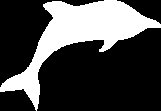
\includegraphics[width=0.3\textwidth]{img/delfin.jpg}
\end{center}

\caption{Silueta de un delfín.}
\label{delfin}
\end{figure}

Así pues, en este capítulo se explicará la investigación realizada para tratar de obtener otros descriptores más cercanos al lenguaje cotidiano, utilizando la lógica difusa. Se introduce además una sección para introducir los conceptos básicos de la lógica difusa.\\

Destacar que no se trata de resolver el problema completo. Se deja a un lado problemas de una entidad propia como el preprocesamiento de las imágenes o la segmentación. Se supone que tenemos imágenes que simplemente son una máscara, donde un 1 indica la presencia del objeto y un 0 su ausencia en un determinado píxel.
%\section{Descriptor clásico: Curvatura}

Intro \todo[color=green!60]{Continuar aquí}

\subsection{Definición matemática}

\subsection{Limitaciones de implementación}
\section{Fundamentos de la lógica difusa}

Es común pensar que una persona que mide un metro con ochenta y cinco centímetros es una persona alta. Pero, ¿cuándo una persona deja de ser alta? ¿Ese cambio es brusco? ¿Todas las personas tienen la misma clasificación de persona alta? En el razonamiento humano usual, no todos los hechos son ciertos o falsos, si no que hay matices e incluso diferentes puntos de vista. Se puede considerar que la información puede ser:

\begin{itemize}
\item \textbf{Incompleta:} Describe parcialmente la realidad.
\item \textbf{Imprecisa:} El valor de una variable se encuentra en un conjunto de valores pero no podemos precisar cual es.
\item \textbf{Incierta:} No tenemos total certeza de que la información sea verdadera.
\end{itemize}

Aún así, el ser humano utiliza estos conceptos imprecisos para razonar, proporcionando a las personas una gran capacidad de razonamiento, y de adaptar ese razonamiento a la situación.\\

Han habido varios intentos de modelizar este fenómeno. Entre ellos, encontramos la Teoría de Conjuntos Difusos, formulada por Lofti A. Zadeh en 1965\cite{Zadeh-Fuzzy-1965}. Este matemático e ingeniero azerbaiyano, basó la lógica difusa en la teoría de conjuntos ordinaria, añadiendo a esta un grado de pertenencia de los elementos al conjunto, en vez de la información binaria de los conjuntos ordinarios, es decir, si un elemento pertenece o no al conjunto sin niveles intermedios.\\

Esta breve introducción a la lógica difusa de Zadeh describirá los conceptos necesarios para poder definir en la siguiente sección propiedades difusas sobre las formas. En concreto se tratará la definición de conjunto difuso y las operaciones básicas con conjuntos difusos.\\

\subsection{Conjuntos difusos}

Un conjunto difuso sobre un universo X es una generalización del concepto clásico de conjunto en el que la función que indica si un elemento pertenece o no al conjunto, la función indicadora, tiene como rango el intervalo real [0,1], en vez del conjunto {0,1}. Por tanto, el conjunto difuso $A$ viene descrito por la función indicadora $\mu_A$:

\[
\ \mu_A : X \longrightarrow [0,1].
\]

En el contexto de la teoría de subconjuntos difusos, se denomina función de pertenencia a la función indicadora. Por lo general, se suele identificar al conjunto difuso con su función de pertenencia. Seguiremos la siguiente notación:

\[
\ A : X \longrightarrow [0,1]
\]

donde, siendo $x \in X$, $A(x)$ representa el grado de pertenencia del elemento $x$ al conjunto difuso $A$.\\

Algunos conceptos básicos sobre conjuntos difusos son:

\begin{itemize}
\item Un conjunto difuso $A$ se dice \textit{normal} si existe al menos un $x \in X$ tal que $A(x)=1$.
\item Se llama \textit{soporte} del conjunto difuso $A$ al conjunto

\[
\ Sop(A) = \lbrace x \in X | A(x) > 0 \rbrace.
\] 
\item Se llama \textit{núcleo} del conjunto difuso $A$ al conjunto

\[
\ Ker(A) = \lbrace x \in X | A(x) = 1 \rbrace.
\] 
\end{itemize}

\subsection{Operaciones básicas con conjuntos difusos}

La extensión de los conjuntos usuales a conjuntos difusos no tendría sentido sin la existencia de operadores básicos para los conjuntos difusos. Por tanto, se pretende extender también de las operaciones principales sobre conjuntos. Las extensiones pueden realizarse de diversas formas, con la condición de que deben comportarse como los operadores ordinarios cuando los conjuntos implicados son ordinarios. Las familias de operadores difusos más importantes son las \textit{t}-normas que extienden a las uniones, las \textit{t}-conormas, que extienden a la unión y las negaciones, que extienden al complemento.\\

\subsubsection{Operadores de intersección: \textit{t}-normas}

Una \textit{t}-norma es una función

\[
\ i: [0,1] \times [0,1] \longrightarrow [0,1]
\]

que verifica las siguientes propiedades para todo $a,b,c \in [0,1]$:

\begin{itemize}
\item \textbf{Frontera:} $i(a,1) = a$.
\item \textbf{Monotonía:} $b \leq c \Rightarrow i(a,b) \leq i(a,c)$.
\item \textbf{Conmutatividad:} $i(a,b) = i(b,a)$.
\item \textbf{Asociatividad:} $i(a,i(b,c)) = i(i(a,b),c)$.
\end{itemize}

Dentro de esta familia de funciones, las más utilizadas usualmente son:

\begin{itemize}
\item \textbf{Mínimo:} $i(a,b)= min(a,b)$.
\item \textbf{Producto algebraico:} $i(a,b)= ab$.
\item \textbf{Recta acortada (Lukasiewicz):} $i(a,b)= max(0,a+b-1)$.
\item \textbf{Intersección drástica:} $i(a,b)= \left\lbrace
  \begin{array}{l}
     b \qquad a = 1 \\
     a \qquad b = 1 \\
     0 \qquad \textrm{ en otro caso }
  \end{array}
  \right.$.
\end{itemize}

Gracias a cualquiera de las \textit{t}-normas, podemos definir la intersección de dos conjuntos difusos $A$ y $B$ de la siguiente forma:

\[
\ (A\cap B)(x)= i(A(x),B(x)).
\]

\subsubsection{Operadores de unión: \textit{t}-conormas}

Una \textit{t}-conorma es una función

\[
\ u: [0,1] \times [0,1] \longrightarrow [0,1]
\]

que verifica las siguientes propiedades para todo $a,b,c \in [0,1]$:

\begin{itemize}
\item \textbf{Frontera:} $u(a,0) = a$.
\item \textbf{Monotonía:} $b \leq c \Rightarrow u(a,b) \leq u(a,c)$.
\item \textbf{Conmutatividad:} $u(a,b) = u(b,a)$.
\item \textbf{Asociatividad:} $u(a,u(b,c)) = u(u(a,b),c)$.
\end{itemize}

Dentro de la familia de funciones de las \textit{t}-conormas, las más utilizadas usualmente son:

\begin{itemize}
\item \textbf{Máximo:} $i(a,b)= max(a,b)$.
\item \textbf{Suma algebraica:} $u(a,b)= a+b-ab$.
\item \textbf{Suma acortada (Lukasiewicz):} $u(a,b)= min(1,a+b)$.
\item \textbf{Intersección drástica:} $u(a,b)= \left\lbrace
  \begin{array}{l}
     b \qquad a = 0 \\
     a \qquad b = 0 \\
     1 \qquad \textrm{ en otro caso }
  \end{array}
  \right.$.
\end{itemize}

Gracias a cualquiera de las \textit{t}-conormas, podemos definir la unión de dos conjuntos difusos $A$ y $B$ de la siguiente forma:

\[
\ (A \cup B)(x)= u(A(x),B(x)).
\]

\subsubsection{Operadores de complemento: negaciones}

Una negación es una función

\[
\ c: [0,1] \longrightarrow [0,1]
\]

que verifica las siguientes propiedades para todo $a,b \in [0,1]$:
\begin{itemize}
\item \textbf{Frontera:} $c(0) = 1$ y $c(1) = 0$.
\item \textbf{Monotonía:} $a \leq b \Rightarrow c(b) \leq c(a)$.
\end{itemize}

Dentro de la familia de funciones de las \textit{t}-conormas, las más utilizadas usualmente son:

\begin{itemize}
\item \textbf{Negación estándar:} $c(a)= 1-a$.
\item \textbf{Negación umbral:} $c(a)= \left\lbrace
  \begin{array}{l}
     1 \qquad a \geq t \\
     0 \qquad a < t \\
  \end{array}
  \right. , \textrm{con } t\in (0,1]$.
\end{itemize}

Gracias a cualquiera de las negaciones, podemos definir el complemento de un conjunto difusos $A$ de la siguiente forma:

\[
\ \bar{A}(x)= c(A(x)).
\]

Normalmente, dentro de las negaciones, se elige la negación estándar por sus buenas propiedades, como por ejemplo ser continua e involutiva, es decir, $c\left(c\left(a\right)\right)=a$, para todo $a \in [0,1]$ .

\subsubsection{Propiedades de los operadores estándar}

El operador estándar de intersección, el mínimo, tiene la interesante propiedad de producir la mayor la función de pertenencia de todas las \textit{t}-normas \cite{Ross}. De modo similar, el operadodr estándar de unión, el máximo, tiene la propiedad de producir la menor función de pertenencia de todas las \textit{t}-conormas. Estas propiedades tienen su importancia ya que previenen del empeoramiento de los errores en los operandos. La mayoría de otras \textit{t}-normas y \textit{t}-conormas no tienen esta ventaja.\\

Utilizando los operadores estándar podemos encontrar propiedades adicionales, similares a las que cumplen los conjuntos ordinarios. Destacar la propiedad distriburiva y las leyes de De Morgan. Siendo $A$, $B$ y $C$ conjuntos difusos:

\begin{itemize}
\item \textbf{Leyes de De Morgan:}
\[
\ \overline{A \cup B} = \overline{A} \cap \overline{B}
\]
\[
\ \overline{A \cap B} = \overline{A} \cup \overline{B}
\]
\item \textbf{Propiedad distributiva:}
\[
\ C \cap \left( A \cup B \right) = \left(C \cap A \right) \cup \left(C \cap B \right)
\]
\[
\ C \cup \left( A \cap B \right) = \left(C \cup A \right) \cap \left(C \cup B \right)
\]
\end{itemize}

Pero no podemos obtener todas las propiedades usuales de los conjuntos ordinarios. Por ejemplo, siendo $A$ un conjunto difuso, las propiedades

\[
\ A \cup \overline{A} = X
\]
\[
\ A \cap \overline{A} = \emptyset
\]

no se cumplen. Dado $x \in X$ y supongamos que $A(x)=\frac{1}{2}$, se cumple $\left( A \cup \overline{A} \right) (x) = \left( A \cap \overline{A} \right) (x) = A(x)$. Por tanto, tenemos un contrajemplo, que nos hace descartar las propiedades anteriores.\\

\subsection{Modificadores lingüísticos}

En el habla, utilizamos adjetivos que alteran la intensidad de una categoría. Por ejemplo, ``muy altos'' modifica la categoría ``altos'' en pos de hacerla más restrictiva, quedándonos únicamente con las personas realmente altas. En la lógica difusa, se crean unos operadores, llamados modificadores lingüísticos, que permiten adaptar esta realidad, realzando valores de la función de pertenencia o haciéndola más o menos permisiva.\\

Se pueden definir muchos modificadores lingüísticos. Vamos a mostrar algunos de los más básicos. Sea $\mu_A$ la función de pertenencia de un conjunto difuso, se definen los siguientes modificadores lingüísticos:

\begin{itemize}
\item \textbf{``Muy'': }$\mu_A = \mu_A^2$.
\item \textbf{``Muy muy'': }$\mu_A = \mu_A^4$.
\item \textbf{``Más'': }$\mu_A = \mu_A^{1.25}$.
\item \textbf{`Un poco'': }$\mu_A = \sqrt{\mu_A}$.
\item \textbf{``Menos'': }$\mu_A = \mu_A^{0.75}$.
\end{itemize}

Los tres primeros forman parte de los modificadores lingüísticos de concentración. Se llaman así ya que reducen mucho la función de pertenencia de los elementos que tienen una baja pertenencia al conjunto, dejando casi sin alterar los elementos que tienen un alto valor de función de pertenencia, consiguiendo un efecto de concentración en torno a los valores que mejor cumplen la condición del conjunto difuso. De manera opuesta, los dos últimos modificadores lingüísticos se conocen como de dilatación.\\

En la teoría de conjuntos difusos podemos encontrar muchos más modificadores lingüísticos y categorías de los mismos.\\

\section{Modelado de formas con conjuntos difusos}

Los descriptores relativos a formas hasta la fecha definen propiedades matemáticas de la misma, pero no tratan de definirla usando conceptos. La curvatura, uno de los descriptores más utilizados es buena muestra de ello. Pese a ser un concepto matemático común, no nos aporta ningún tipo de información, solo un conjunto de valores que la representa. Utilizando la lógica difusa, se puede tratar de modelar conceptos lingüísticos comunes en el habla, tales como si un objeto es alargado o redondeado, adaptándose a las posibles imprecisiones del mundo real.\\

En una primera incursión en este tema\cite{JChamorro}, se trata de definir los conceptos más básicos sobre contornos, la ``linealidad'', la ``curvacidad'' y la ``verticidad'', que servirán de base para futuras propiedades. En este trabajo se muestran la definición de dichos conceptos, además de algunas correcciones y mejoras aportadas al artículo original.\\

\subsection{Linealidad}

\subsubsection{Definición}
La linealidad define en que grado un segmento del contorno es una línea.\\

Sea $ C = \left\lbrace p_i = \left( x_i,y_i\right) \right\rbrace_{0\leq i\leq n}$ un contorno definido como un conjunto ordenado cíclico. Sea $S^C_{ij} = \left\lbrace p_k \in C \right\rbrace_{i \leq k \leq j}$ y $\Theta^C = \left\lbrace S^C_{ij}\right\rbrace_{i \neq j}$.\\

Definimos la linealidad a través de un conjunto difuso:\\

\[
\ \tilde{L}:\Theta^C \rightarrow \left[ 0,1 \right]
\]

Cuya función de pertenencia es:\\

\[
\ \tilde{L} \left(S^C_{ij}\right) = A \left( 1-\frac{\sum^j_{k=i} \parallel p_k - \widehat{p}_k \parallel}{\sum^j_{k=i} \parallel p_k - \overline{p}_{S^C_{ij}} \parallel} \right)
\]

Donde $\parallel p_k - \widehat{p}_k \parallel$ es la distancia entre el punto $p^k$ y la recta de regresión de los puntos del segmento, $\parallel p_k - \overline{p}_{S^C_{ij}} \parallel$ es la distancia entre el punto $p^k$ y la media de los puntos del segmento $\overline{p}_{S^C_{ij}}$ y $A$ es una función de ajuste.\\

Dado que los puntos $\widehat{p}_k$ son obtenidos a través de la proyección a una recta de regresión, el numerador de la fórmula será siempre menor o igual que el denominador. Obtenemos por tanto un valor entre 0 y 1, valiendo 0 si el ajuste de la recta de regresión es perfecto ---es decir, el segmento es una recta perfecta--- y 1 en el peor de los casos. Restando este valor a 1, obtenemos lo que buscábamos, un indicador que nos devuelva 1 si estamos ante una recta y vaya bajando hasta el 0, según los puntos del contorno se vayan alejando de una recta.\\

Sin embargo, el rango obtenido al aplicarlo a imágenes reales no varía en todo el intervalo $\left[ 0,1 \right]$, lo que hace necesaria la introducción de la función de ajuste $A$. Para la selección de dicha función, se diseñó un experimento en el que se transformaba una línea recta en una semicircunferencia. La fórmula para la creación de estos segmentos intermedios es:\\

\[
\ y = (1-p)+ p \sqrt{1-x^2}
\]

Donde $p$ es el porcentaje de semicircunferencia de la forma. En la figura \ref{fig2} podemos encontrar los resultados de calcular la linealidad sin ningún tipo de ajuste, con 100 pasos intermedios.\\

\begin{figure}[H]
\begin{center}

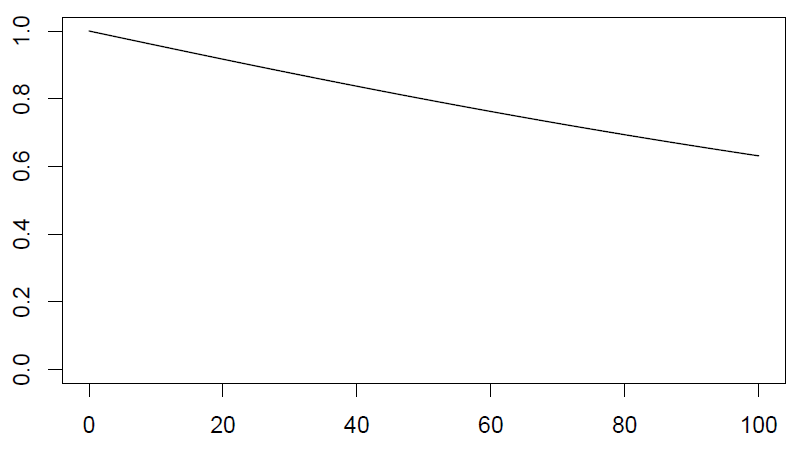
\includegraphics[width=0.9\textwidth]{img/linea-curva.png}
\end{center}

\caption{Linealidad sin ajuste.}
\label{fig2}
\end{figure}

Una primera aproximación fue pensar en funciones de ajuste del tipo $A(x) = x^q$ con $q \in \mathcal{R}^+$. Pero como podemos ver en la figura \ref{fig3}, necesitamos un $q$ grande para llevar los valores a un valor cercano a 0, lo que deforma la gráfica.\\

\begin{figure}[H]
\begin{center}

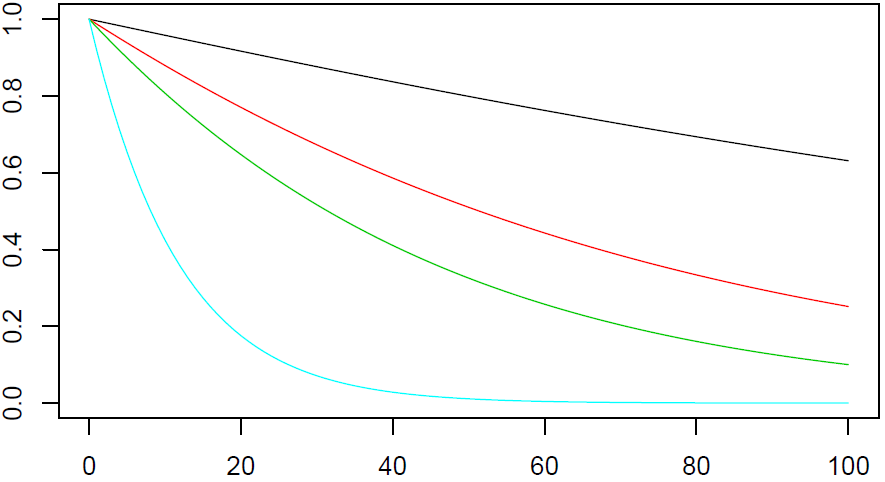
\includegraphics[width=0.9\textwidth]{img/Ajuste-q.png}
\end{center}

\caption{Linealidad con ajuste tipo potencias. q = 3,5,20.}
\label{fig3}
\end{figure}

Por tanto, se pasó a un ajuste de tipo "cambio de rango". Tomamos como posibles A la familia de funciones:\\

\[
\ A(x,\alpha) = \texttt{max}\left(\frac{x-\alpha}{1-\alpha} ,0\right)
\]

Queda libre el ajuste de $\alpha$. Este valor está asociado al ángulo del arco de circunferencia que consideramos que ya no es una línea. En la figura \ref{fig4} tenemos una gráfica que relaciona el ángulo del arco de circunferencia con su valor de $\alpha$.\\

\begin{figure}[H]
\begin{center}

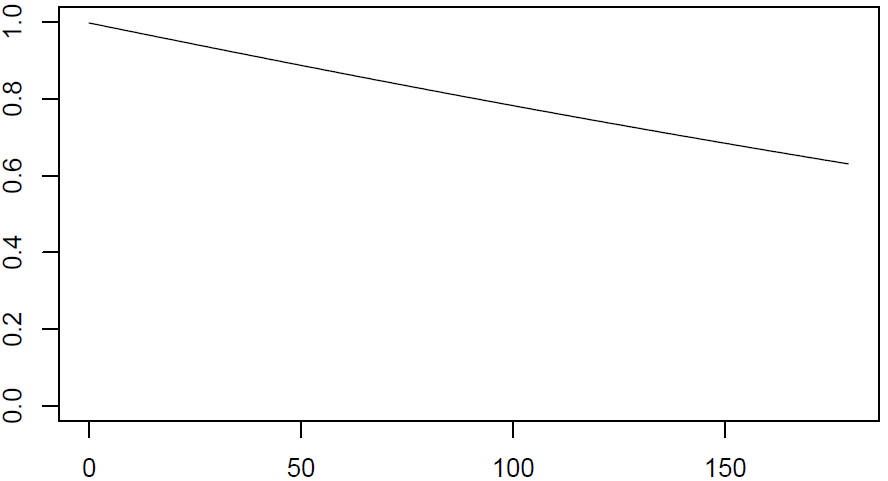
\includegraphics[width=0.9\textwidth]{img/experimento-angulo.png}
\end{center}

\caption{Linealidad de los arcos de circunferencia.}
\label{fig4}
\end{figure}

Podemos aproximar la línea de la figura \ref{fig4} para obtener una relación rápida entre el arco de circunferencia que consideramos que ya no es una linea y el $\alpha$ que debemos fijar. Obtenemos la siguiente función:\\

\[
\ \alpha(\Theta) = 1- \frac{0.37}{\pi} \Theta
\]

Utilizando $\alpha = 0.63$ en el experimento de la figura \ref{fig2}, obtenemos el ajuste de la figura \ref{fig5}, que se comporta de manera lineal y que cubre de manera efectiva el rango [0,1].\\


\begin{figure}[H]
\begin{center}

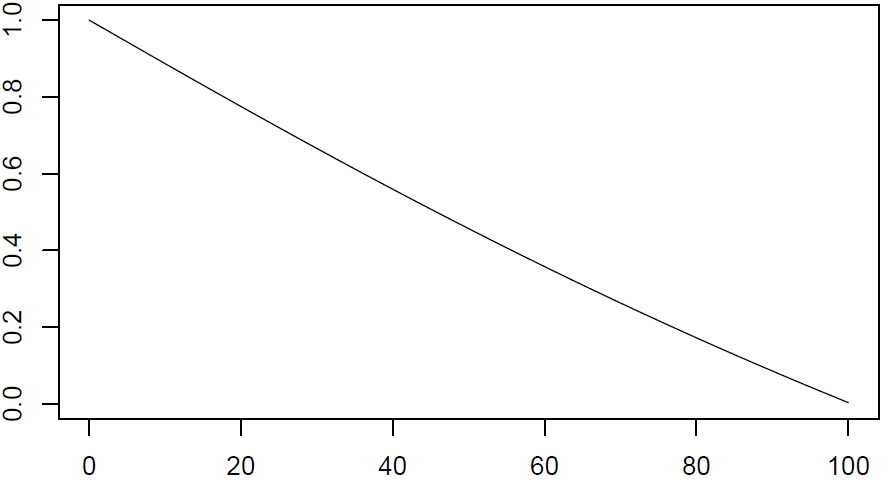
\includegraphics[width=0.9\textwidth]{img/Ajuste-alfa.png}
\end{center}

\caption{Linealidad de la figura \ref{fig2} ajustada.}
\label{fig5}
\end{figure}

\subsubsection{Resultados}

Utilizaremos para ver la influencia del valor $\alpha$ la siguiente figura:\\

\begin{figure}[H]
\begin{center}


\includegraphics[width=0.3\textwidth]{img/device3-1.png}
\end{center}

\caption{Cuadrado redondeado.}
\label{cuadrado-red}
\end{figure}

Podemos ver en la figura \ref{fig6}, que si tomamos un $\alpha$ asociado a un ángulo pequeño, en este ejemplo 45º, vemos que obtenemos unos resultados que varían de manera muy drástica.

\begin{figure}[H]
\begin{center}

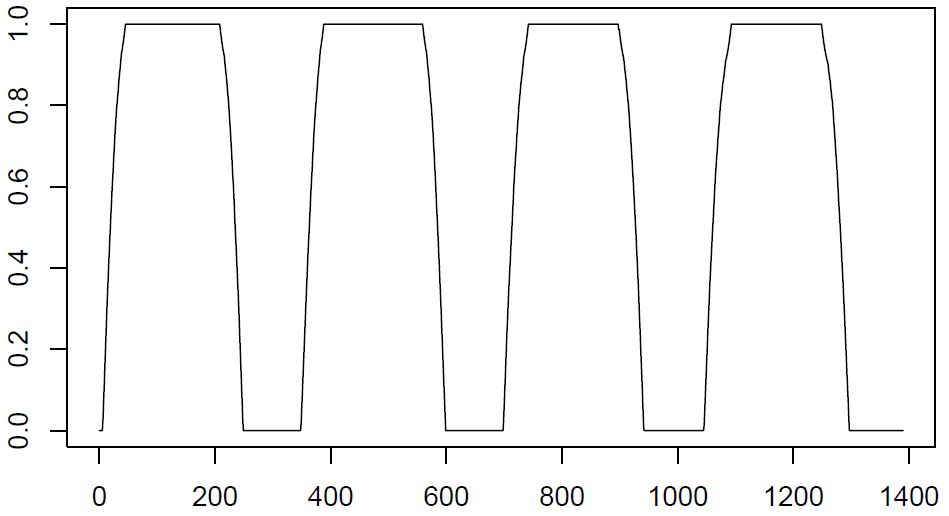
\includegraphics[width=0.9\textwidth]{img/lin-dev3-1-limpio-09075.png}
\end{center}

\caption{$\Theta = 45$ ($\alpha = 0.9075$).}
\label{fig6}
\end{figure}

De modo similar, en la figura \ref{fig7} podemos ver que si el ángulo seleccionado es demasiado permisivo, en el ejemplo 180º, se obtienen valores que nunca alcanzan el 0.\\

\begin{figure}[H]
\begin{center}

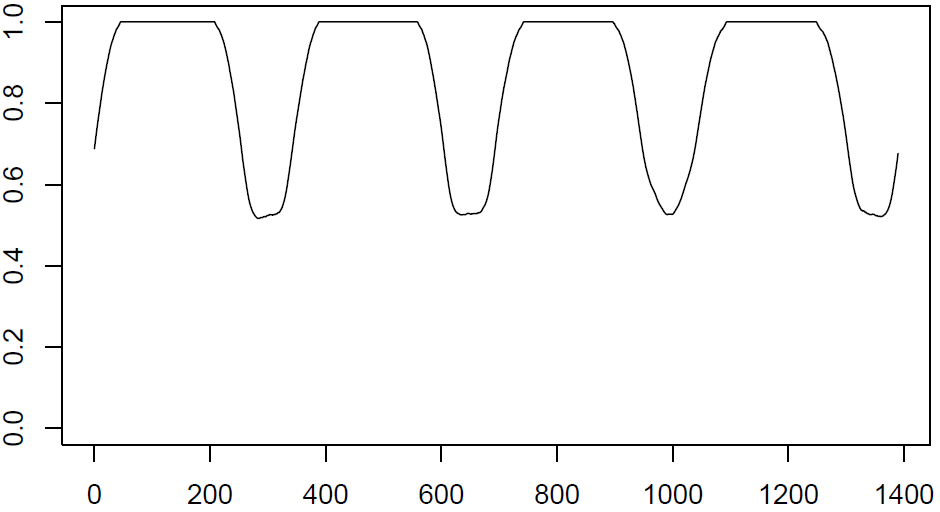
\includegraphics[width=0.9\textwidth]{img/lin-dev3-1-limpio-063.png}
\end{center}

\caption{$\Theta = 180$ ($\alpha = 0.63$).}
\label{fig7}
\end{figure}

En la figura \ref{fig8}, ajustando $\alpha$ a un valor intermedio, conseguimos un ajuste más apropiado para esta figura.\\

\begin{figure}[H]
\begin{center}

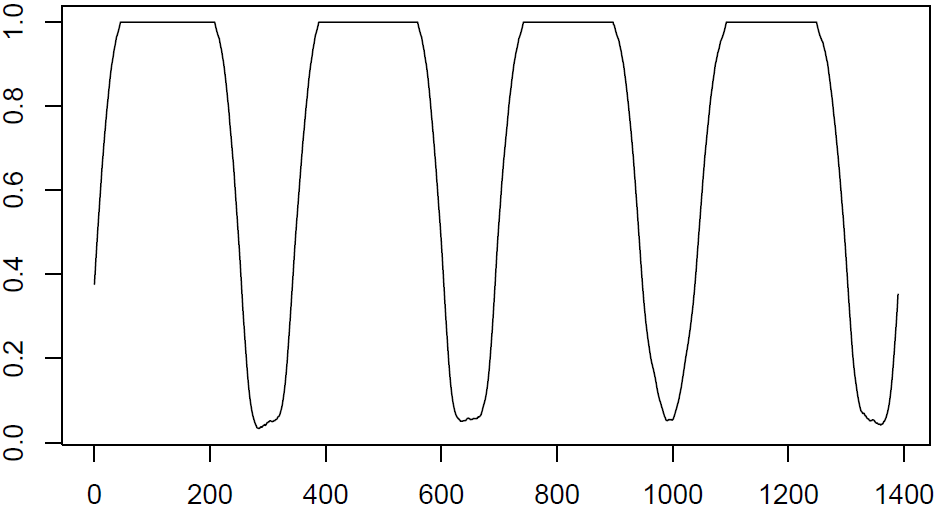
\includegraphics[width=0.9\textwidth]{img/lin-dev3-1-limpio-0815.png}
\end{center}

\caption{$\Theta = 90$ ($\alpha = 0.815$).}
\label{fig8}
\end{figure}

Se extrae por tanto que tenemos un buen comportamiento de esta primera propiedad, la linealidad, quedando libre el parámetro $\alpha$ para ser ajustado según las necesidades del problema a tratar, o dicho de otro modo, para poder ajustar lo que se considera que no es lineal.\\

\subsection{Curvacidad}


\subsubsection{Definición}

Entendemos la curvacidad como el grado en el que el segmento de un contorno es una curva. Se define como el opuesto de la linealidad, es decir:\\

\[
\ \tilde{U}(S^C_{ij}) = 1 - \tilde{L}^C_{ij}
\]
 
\subsubsection{Resultados}

Primero, veremos la gráfica de la curvacidad del cuadrado redondeado de la figura \ref{cuadrado-red}.

\begin{figure}[H]
\begin{center}
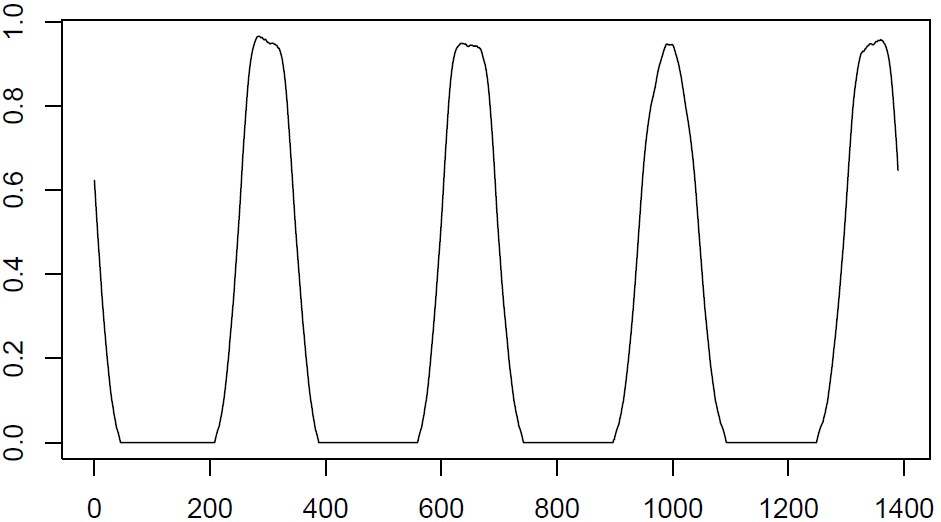
\includegraphics[width=0.9\textwidth]{img/nolin-dev3-1-limpio-0815.png}
\end{center}

\caption{Curvacidad de la imagen cuadrado redondeado.}
\label{fig9}
\end{figure}

Podemos ver en la figura \ref{fig9} que actúa como esperábamos, obteniendo 4 valores altos, que corresponden a las 4 esquinas de la figura. Además nos lleva a pensar que se tienen que comportar de manera similar a la curvatura.\\

En la figura \ref{fig10} podemos ver la gráfica de la curvacidad de una forma natural. Podemos observar que el comportamiento es adecuado, lo que reafirma el buen comportamiento de nuestras propiedades.\\

Sin embargo, podemos ver que todos los picos asociados a los giros son positivos. Esto muestra la desventaja de este modelo con respecto a la curvatura, que sí nos indica el sentido del giro mediante el signo del valor.\\

\begin{figure}[H]
\begin{center}

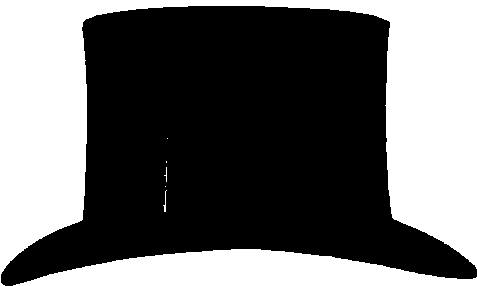
\includegraphics[width=0.3\textwidth]{img/hat-7.png}
\newline
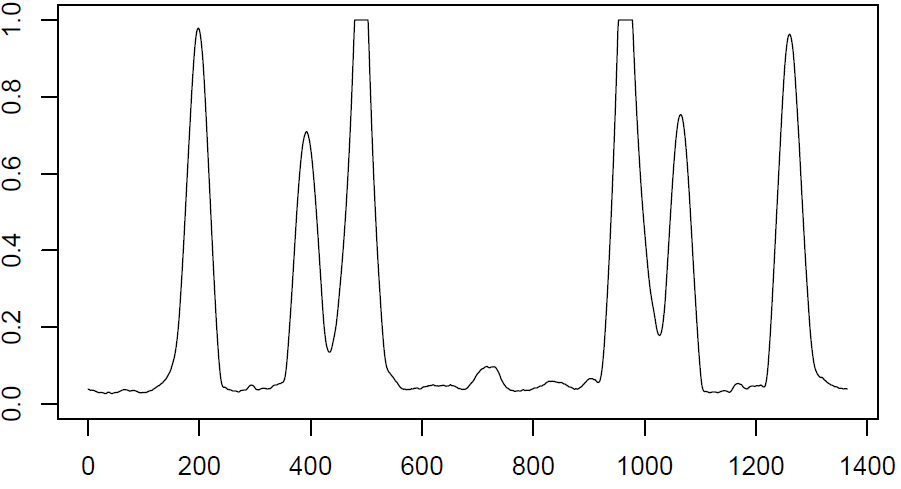
\includegraphics[width=0.9\textwidth]{img/nolin-hat-7.png}
\end{center}

\caption{Curvacidad de la imagen sombrero.}
\label{fig10}
\end{figure}


Evidentemente, al ser la propiedad opuesta a la linealidad, tiene la misma dependencia del parámetro $\alpha$, permitiendo ajustar que se considera curva según las necesidades del problema.\\

\subsection{Verticidad}

\subsubsection{Definición}
La verticidad describe el grado en el que un punto del contorno es un vértice.\\

En un vértice, se cumplen los siguiente hechos:
\begin{itemize}
\item Es el punto donde dos rectas se cortan, por tanto se espera una alta linealidad a izquierda y derecha del punto.
\item Las líneas que se cruzan en el vértice forman un ángulo, luego la linealidad en el punto se espera que sea baja. O dicho en otras palabras, que la curvacidad sea alta.
\end{itemize}

Por tanto, utilizando los conceptos creados anteriormente, se modela la verticidad como:\\

\[
\ \tilde{V}(C,i) = \otimes \left(\tilde{L}^C_{i-w,i}, \tilde{L}^C_{i,i+w},  \tilde{U}(S^C_{i-w/2,i+w/2})   \right)
\]
Con i el indice del punto en el contorno, $ \otimes $ una t-norma y $w$ el tamaño considerado de segmento. Se pueden añadir modificadores lingüísticos del tipo "muy" para enfatizar el cumplimiento de alguna de las características.

\subsubsection{Resultados}

Primero, veamos su comportamiento con una forma que contiene varios vértices reales y un vértice redondeado.\\

\begin{figure}[H]
\begin{center}


\includegraphics[width=0.3\textwidth]{img/fig4.png}
\newline
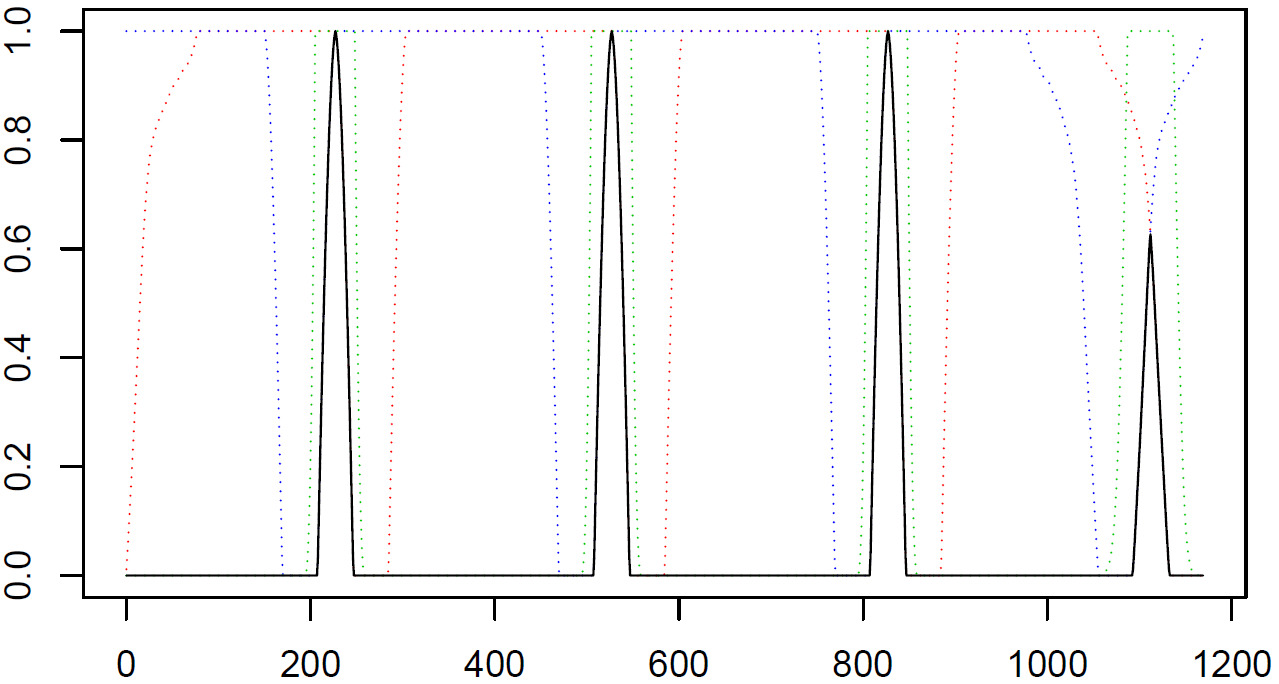
\includegraphics[width=0.9\textwidth]{img/vert-fig04-novvery.png}
\end{center}

\caption{Verticidad cuadrado con una esquina redondeada.}
\label{fig11}
\end{figure}

En la figura \ref{fig11} podemos ver que, efectivamente, nuestro grado de verticidad llega a 1 en los 3 vértices reales que tiene la figura y da un valor menor al vértice redondeado.\\

En la figura \ref{fig12} tenemos la verticidad del cuadrado redondeado. Al tener unas esquinas más redondeadas que en el caso de la figura \ref{fig11}, los valores que obtenemos son mucho menores, como es de esperar.\\

\begin{figure}[H]
\begin{center}


\includegraphics[width=0.3\textwidth]{img/device3-1.png}
\newline
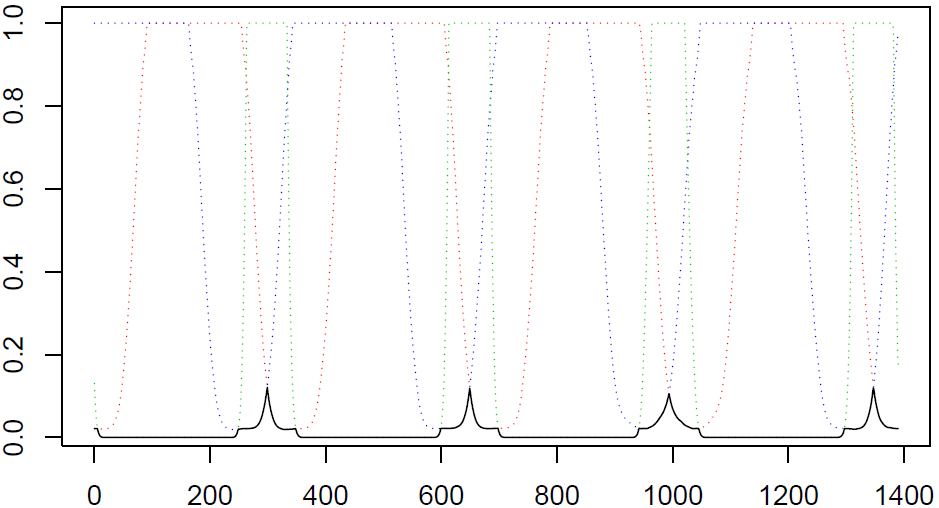
\includegraphics[width=0.9\textwidth]{img/vert-dev3-1-limpio.png}
\end{center}

\caption{Verticidad cuadrado redondeado.}
\label{fig12}
\end{figure}

Por tanto, la verticidad tiene un comportamiento deseable. Destacar que esta propiedad ha sido construida mediante el uso de propiedades más sencillas, intentando siempre utilizar los conceptos difusos para razonar.\\

\todo[color=blue!50]{poner conclusiones de la investigación aquí?}


\chapter{Clasificación Automática}
\label{ch2}
El etiquetado automático de las imágenes es un ámbito de la informática en pleno desarrollo. Pese a que se usan técnicas propias del campo de la visión por computador, los mayores avances se están obteniendo mediante la incorporación de técnicas de aprendizaje automático.\\

Estos avances se deben al desarrollo del llamado ``Deep Learning'', que ha permitido a los investigadores alcanzar buenos resultados en la clasificación en grandes bases de imágenes, como Image-net ~\cite{imagenet_cvpr09}, utilizando un modelo de redes neuronales convolucionales.\\

Se hace necesario por tanto un estudio de las bases del aprendizaje automático y de su problemática para después explicar el funcionamiento del ``Deep Learning'' y el modelo de las redes neuronales convolucionales. Tras esto, se mostrarán los resultados obtenidos con las redes neuronales convolucionales que estarán disponibles en la aplicación final en el desafío lanzado desde Image-net, ImageNet Large Scale Visual Recognition Competition (ILSVRC)~\cite{ILSVRC15}.\\


\section{Fundamentos del Aprendizaje Automático}

Pese a que es fácil reconocer un árbol en una imagen, la descripción precisa de que es un árbol es prácticamente imposible. La tarea se hace aún más difícil cuando tenemos que especificar estos detalles para una computadora. Aún así, se ha conseguido completar esta tarea, gracias al Aprendizaje Automático.\\

El Aprendizaje Automático es la rama de la informática que trata el estudio y la creación de algoritmos que puedan aprender automáticamente de los datos.\\

En esta sección seguiremos fundamentalmente el libro de Abu-Mostafa \cite{Abu-Mostafa:2012:LD:2207825} para la introducción a los conceptos más importantes del Aprendizaje Automático.\\

\subsection{Tipos de Aprendizaje Automático}

La premisa básica del aprendizaje es el uso de un conjunto de oobservaciones para tratar de descubrir el proceso que hay detrás de las mismas. Esto es una premisa muy amplia, por lo que se divide en varios paradigmas, cada uno centrado en diferentes situaciones.\\

En esta apartado se tratarán los paradigmas más importantes, destacando el aprendizaje supervisado ya que es el más estudiado y utilizado, y además es el paradigma en el que encaja la clasificación automática en etiquetas de imágenes, objetivo de este trabajo.\\

\subsubsection{Aprendizaje supervisado}

Cuando el conjunto de datos contiene de manera explícita la salida correcta para el dato, nos encontramos ante un caso de aprendizaje supervisado. Por ejemplo, supongamos una base de datos para el reconocimiento de dígitos escritos a mano. Sería razonable que la base de datos se compusiera de imágenes con ejemplos de dígitos escritos a mano y el dígito escrito en cada imagen, obteniendo un conjunto de parejas imagen y dígito.\\
 
Lo común dentro de este caso es que se presente la base de datos en su totalidad, pero existen otras opciones.\\

Por un lado, encontramos el aprendizaje activo, donde el conjunto de datos se obtiene mediante consultas. En este paradigma, se elige el punto x del espacio de entrada y se obtiene la salida de x. Esto permite una elección estratégica de de los puntos para maximizar el aprendizaje\\

Por otro lado, encontramos el aprendizaje online. En esta ocasión, los datos se presentan de uno en uno. Por ejemplo, este caso se puede dar cuando admitimos nuevos datos durante ejecución, permitiendo la entrada de un dato y su clasificación, adaptando el modelo en consecuencia. También es de utilidad cuando tenemos limitaciones de computación o almacenamiento, permitiendo procesar los datos cuando no podemos procesar la base de datos completa. Destacar que el aprendizaje online puede ser usado en diferentes paradigmas del aprendizaje, y no sólo en el aprendizaje supervisado.\\

\subsubsection{Aprendizaje por refuerzo}

En cuanto no disponemos explícitamente de la salida correcta para un dato, no nos encontramos en el caso del aprendizaje supervisado. Aún así, hay situaciones en las que pese a no tener una salida a priori, podemos tener un grado de acierto de la acción. Por ejemplo, supongamos a un bebe aprendiendo que hacer ante un objeto caliente. El bebe tendría dos opciones, tocar o no tocar el objeto. Si no toca el objeto, la insatisfacción de su curiosidad le producirá algo de mal estar. Si lo toca, el dolor será mayor. Pese a que el objeto no presenta claramente la respuesta al problema del bebe, tras varios intentos aprenderá que es mejor no tocar el objeto.\\

Esto caracteriza el aprendizaje por refuerzo, donde los datos no presentan claramente el resultado, pero si contienen una posible salida junto con una medida de la bondad de la salida, a diferencia del aprendizaje supervisado que contiene únicamente el dato y la salida. Es importante destacar que en el aprendizaje por refuerzo no sabemos la bondad de las demás posibles salidas.\\

El aprendizaje por refuerzo es usado principalmente para aprender a jugar a un juego. Por ejemplo, en una partida de ajedrez tienes que elegir entre un conjunto de movimientos para tomar la mejor acción. Sin embargo, es muy difícil, dada una situación de la partida decidir cuál es la mejor acción, haciendo imposible la generación de un ejemplo para el aprendizaje supervisado. Sin embargo, es muy fácil generar un ejemplo de aprendizaje por refuerzo, simplemente hay que tomar una acción y luego, informar del resultado de la misma. Tras esto, es el algoritmo de aprendizaje por refuerzo el que analiza la información para tratar de encontrar la mejor jugada.\\

\subsubsection{Aprendizaje no supervisado}

El caso del aprendizaje no supervisado es en el que los datos no contienen ninguna información de la salida. En un principio, al no disponer de una salida esperada para los datos, parecería que no es posible aprender nada de los mismos. Sin embargo, este caso incluye el análisis de clúster o clustering. En él se pretende clasificar los datos en diferentes conjuntos o clústers, de manera que en cada conjunto tengamos elementos parecidos entre ellos.\\

Además de su utilidad propia para detectar patrones y estructuras ocultas dentro de los datos, se puede utilizar como fase previa para un proceso de aprendizaje supervisado \todo[color=red!50]{Cita Lecun de la Nature} para mejorar el comportamiento final del sistema.\\

\subsection{Componentes del Aprendizaje Automático}
\subsection{¿Es posible aprender?}
\subsection{Error y ruido}
\subsection{Medidas de bondad del aprendizaje}
\subsection{Sobreaprendizaje}
\section{Fundamentos de las redes neuronales convolucionales}
%Breve introducción

\subsection{Definición de neurona artificial}
\subsection{Redes Neuronales}
\subsection{Back Propagation y Deep Learning}
\subsection{Redes neuronales convolucionales}
\subsection{Comparativa de redes neuronales}

\section{Clasificación automática de imágenes}

En las secciones anteriores se ha explicado las bases del aprendizaje automático y del modelo que se va a utilizar para el objetivo final de la clasificación automática de imágenes. En esta sección se detallarán los componentes principales del sistema final de clasificación adoptado.\\

Por tanto, tenemos que definir los conceptos a aprender y el conjunto de entrenamiento. Así, se describirá la base de datos ``ImageNet''\cite{imagenet_cvpr09} y la competición ILSVRC\cite{ILSVRC15}. Además, se hablará de la librería usada para el entrenamiento, Caffe \cite{jia2014caffe} y el modelo adoptado, una adaptación del modelo Alexnet\cite{NIPS2012_4824}.\\

\subsection{ImageNet e ILSVRC}

ImageNet es una base de datos de imágenes  mantenida por las universidades de Standford y Princeton. Las imágenes se organizan según la jerarquía definida en WordNet. En WordNet, cada concepto se clasifica dentro de un ``conjunto de sinónimos'' determinado, también conocido como ``synset''. ImageNet, por tanto, divide sus imágenes por synsets, teniendo según su página web 14.197.122 imágenes de 21.841 synsets diferentes. Las imágenes pasan un control de calidad y son anotadas por humanos. El objetivo es disponer de una base de datos de alta calidad, que contenga en torno a mil imágenes por concepto dentro de la jerarquía de Wordnet, que tiene en la actualidad más de 100.000 synsets.\\

El fin de esta base de datos es facilitar la tarea de la investigación en el campo de las imágenes y la visión por computador. Es claro que para poder realizar una buena investigación, se necesita una buena fuente de información. Por tanto, para poder afrontar el problema de la clasificación de imágenes a gran escala, se hace necesaria una base de datos a gran escala. Con la motivación de crear una gran base de datos para este tipo de problemas, nació ImageNet.\\

ImageNet no posee los derechos de las imágenes contenidas en la base de datos. Por ello, lo único que pueden dar de manera abierta es el enlace a la imagen, de manera similar a los buscadores de imágenes. Sin embargo, las base de datos está completamente disponible para investigadores y docentes que usen las imágenes con fines no comerciales.\\

Dentro de ImageNet, existe una competición llamada ImageNet Large Scale Visual Recognition Competition (ILSVRC). Aunque ahora la competición tiene varias modalidades distintas para competir, desde sus inicios el problema principal ha sido el de clasificar imágenes dentro de 1.000 categorías distintas. Estas categorías representan un marco muy amplio, podemos encontrar desde material de oficina como impresoras a una gran variedad de animales. Dada esta variedad tan amplia, y a ser un problema conocido, se ha tomado los datos de esta competición, en concreto la edición de 2012, para realizar el aprendizaje de nuestro modelo.\\

\subsection{Información del aprendizaje}

Para el entrenamiento del clasificador utilizamos la librería Caffe \cite{jia2014caffe}. Caffe es un framework de deep learning, desarrollado por el  Berkeley Vision and Learning Center (BVLC). Además, tiene una amplia comunidad que ayuda a mantener el código del proyecto y los modelos de acuerdo al estado del arte. Una de sus principales ventajas es la sencillez. Todas las opciones de optimización se hacen con simples cambios de configuración, sin tener que programar nada. Los modelos de redes se definen en un fichero simple, donde solamente hay que definir el tipo y la estructura de cada capa. Además, es tambíen una librería rápida, permitiendo beneficiarse del uso de tarjetas gráficas junto con las librerías CUDA y CuDNN de Nvidia.\\

\begin{figure}[H]
\begin{center}

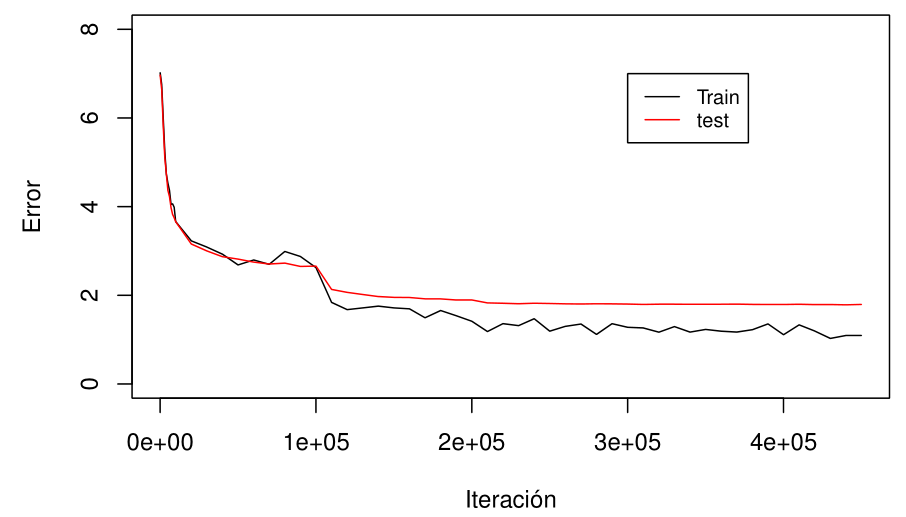
\includegraphics[width=0.9\textwidth]{img/resultados.png}
\end{center}

\caption{Resultados del entrenamiento.}
\label{resultados}
\end{figure}

El modelo entrenado fue caffenet, una versión modificada de la red Alexnet, ganadora de la competición ILSVRC en el año 2012, y que superó con creces todos los resultados de la competición, al ser la primera red en adoptar el modelo de las redes neuronales convolucionales. El entrenamiento se ejecutó sobre una gráfica GTX 1080 de Nvidia, usando las últimas versiones disponibles de las librerías CUDA y CuDNN. El proceso de aprendizaje duró más de 2 días, lastrado por bloqueos de I/O, aunque la gravedad es estos bloqueos fue menor.\\
 
En la figura \ref{resultados} podemos ver el desarrollo de los error de entrenamiento y de test de la red. Como se podría esperar, ambos errores son muy similares hasta un punto donde el error de entrenamiento empieza a bajar más que el de test. Esto empieza a mostrar signos del sobreentreno, pues muestra mejores resultados de entrenamiento que de test, cuando se esperarían resultados parecidos. Aún así, no se observa un efecto catastrófico de sobreentrenamiento. Esto puede deberse a que quizás todo el control de la dimensionalidad de las redes neuronales convolucionales consigue reducir efectivamente los problemas de sobreentrenamiento.  Los pesos seleccionados son los correspondientes a la iteración 370.000, con un error de test 1.80 y un porcentaje de acierto en la clasificación del 57.92\%.


\chapter{Aplicación}
\label{ch3}
\input{tex/aplicacion/aplicacion}

\chapter{Conclusiones y vías futuras}
\label{ch4}
\section{Conclusiones}

La construcción de este tipo de aplicaciones, tiene un gran futuro y seguro que en poco tiempo, grandes empresas del sector lanzarán funcionalidades de este estilo. Quizás, el mayor problema lo encontramos en las técnicas de aprendizaje automático que, pese a ser muy potentes, todavía son débiles y no llegan al nivel de un humano en la clasificación de imágenes. Esta falta de acierto hace que aún sea un poco pronto y aventurado su uso en una aplicación comercial. Además, un fallo en este tipo de aplicaciones puede, por ejemplo, suponer una ofensa para los usuarios, clasificando mal el genero de los mismos, por ejemplo. Esta limitación es la que pone el freno a estas aplicaciones. 

El proyecto ha conseguido finalizar los objetivos planteados en un primer momento. La aplicación desarrollada es un pequeño prototipo, capaz de recuperar información utilizando para ellos un amplio abanico de términos lingüísticos de alto nivel. La extracción de información se realiza mediante una red neuronal convolucional, una de los modelos que mejor resultado han conseguido en el campo de la clasificación automática de imágenes.\\

El objetivo de crear un sistema basado en la lógica difusa para clasificar formas en base a términos lingüísticos ha sido alcanzado parcialmente. Si bien no se ha llegado a completar su desarrollo, se han planteado las bases para su finalización en el futuro y se ha usado como un descriptor para el prototipo.\\

Además, se ha llevado un estudio de los fundamentos teóricos de los dos modelos utilizados.\\

\section{Trabajo Futuro}

La aplicación desarrollada es de un carácter simple, y podría ser mejorada en varios aspectos. Por una parte, se podría ver beneficiada de una mejora a nivel visual, mejorando la interfaz para el usuario. Por otro lado, se podría aumentar la funcionalidad, aumentando por ejemplo el número de clasificadores integrados en la misma o el número de características por las que buscar.\\

Además, el método de almacenamiento de la información es bastante simple. Para conseguir que el sistema sea escalable, se debería de guardar dicha información dentro de una base de datos adecuada, para facilitar las búsquedas y el almacenamiento.\\

Otro punto a trabajar, es la fuerte dependencia del prototipo a la librería Caffe. Eliminar esta dependencia por otra que tenga una mejor integración en el lenguaje Java o eliminar totalmente la dependencia con la creación de un módulo propio sería otra vía de mejora del proyecto.\\

Por supuesto, la creación y diseño de nuevos clasificadores que mejoren los resultados del clasificador de la aplicación es también una vía de futuro. Este es un campo donde varias empresas fuertes del sector están realizando grandes esfuerzos. La investigación en este campo sigue siendo importante y se encuentra actualmente al alza.\\

En cuanto a los descriptores de formas, queda mucho trabajo por hacer. Hay que hacer un estudio más profundo de distintas variables, por ejemplo el tamaño de ventana y buscar técnicas para adaptarlo automáticamente según la figura. Además hay que avanzar en la descripción de formas a partir de ellos, para poder llegar al objetivo de transformar una forma en conceptos del tipo triángulo, cuadrado, etcétera. Incluso, se podría hacer una comparación con las medidas usuales, por ejemplo la curvatura, para ver si se mejora el funcionamiento de técnicas tales como la búsqueda de puntos de interés y la reconstrucción de las imágenes a partir de dichos puntos y la información que tenemos de ellos.\\


\bibliographystyle{unsrt}
\bibliography{tex/bibliografia}
\addcontentsline{toc}{chapter}{Bibliografía}

\end{document}
